\begin{section}{$\pi$-Conjugated Polymers and Polythiophene}
\paragraph{Conjugated polymers} Conjugated polymers are attracting great interest and research effort due to their semiconducting properties, suitable to substitute classical inorganic semiconductors (for example silicon) in lightweight and flexible devices. Inconveniently conjugated polymers are generally insoluble and infusible materials due to their rigidity and to strong intermolecular $\pi-\pi$ stacking interactions. In order to increase the solubility and to modulate the material properties, conjugated polymers have been substituted with appropriate side groups.

\begin{SCfigure}[][tbp]%conjugated_polymers
\centering
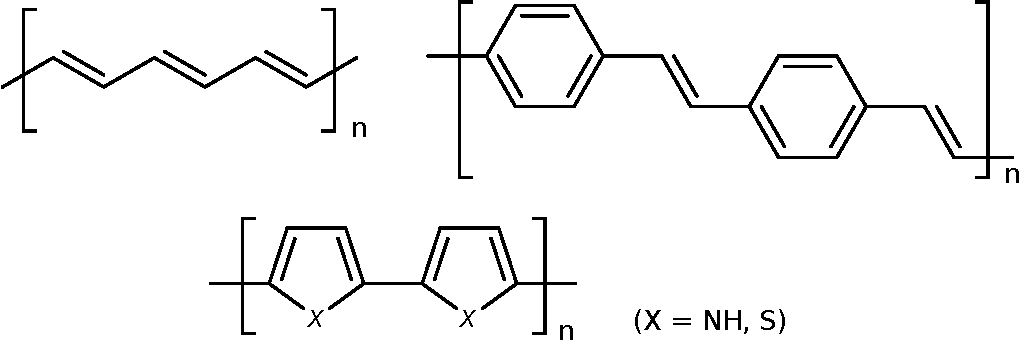
\includegraphics[scale=0.6]{conjugated_polymers.pdf}
\caption{Some conjugated polymers.}
\label{fig:conjugated_polymers}
\end{SCfigure}

\paragraph{Polythiophene} Polythiophene was the first material to give good results in a broad spectrum of applications such as light emitting diodes,\superfootcite{Ohmori1991} field effect transistors\superfootcite{Garnier1994} and organic solar cells\superfootcite{ADMA:ADMA19950070709} due to its convenient optical and electrical properties as well as excellent thermal and chemical stability. Polythiophene properties can be tuned via an easy substitution at one or two of the $\beta$ positions of the thiophene ring and these side chains can add solubility and processability properties to poly\-thio\-phenes. 
The polymer electronic and electrochemical properties can be tuned by varying the electronic properties of the side groups. Also the bulkiness of these groups is important, it can lead, via reciprocal steric repulsion, to a twist in the poly\-thiophenic backbone, reducing the conjugation length and ruining the semiconducting properties. In order to minimize steric interactions, usually only one side group per thiophene unit is bonded in $\beta$ position, doing so the monomeric unit results to be asymmetric. 

\begin{figure}[tbp]%regioregolare-regioirregolare
\begin{subfigure}[b]{0.47\textwidth}
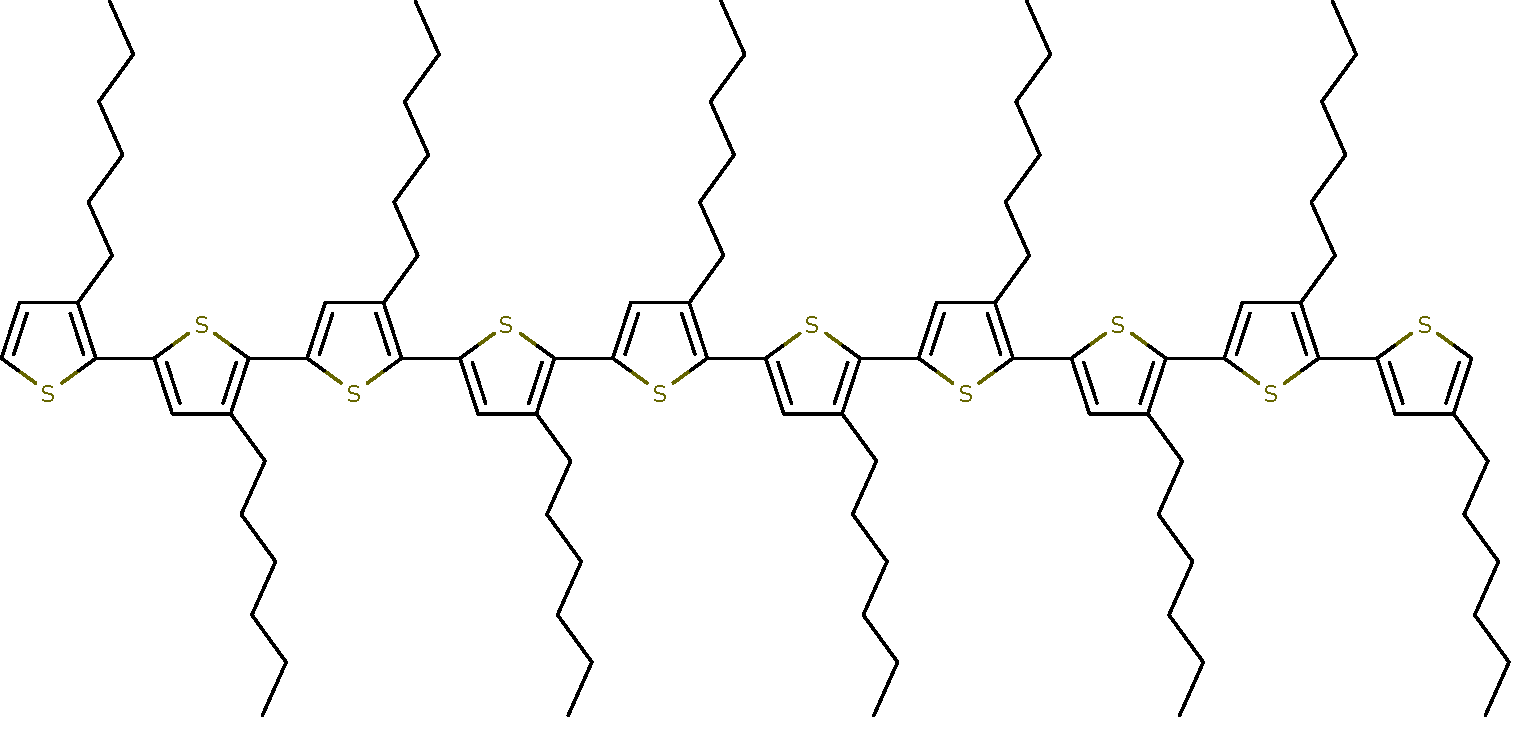
\includegraphics[width=1\textwidth]{regioregolare.pdf}
\subcaption{regioregular}\label{fig:regioregolare}
\end{subfigure}
\qquad
\begin{subfigure}[b]{0.47\textwidth}
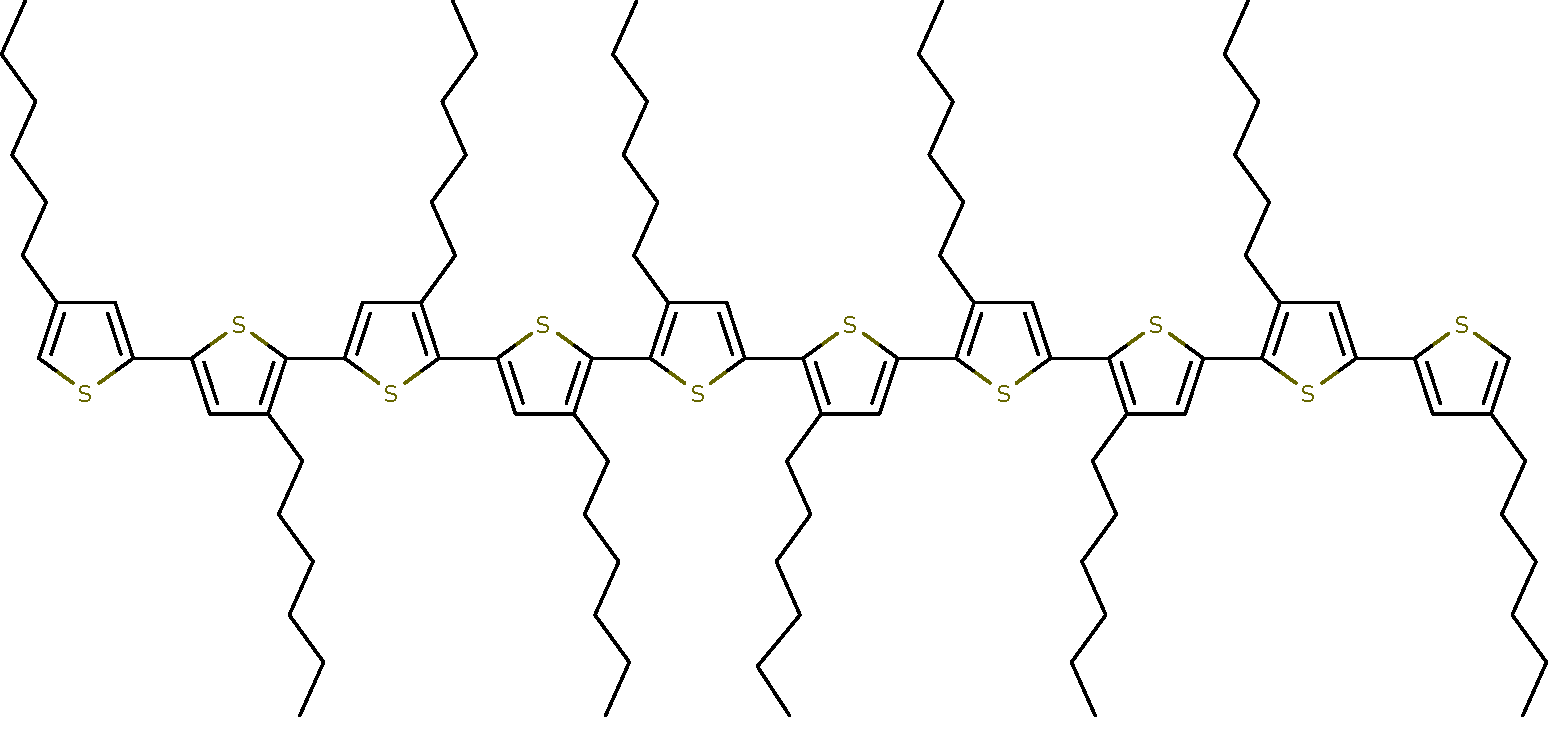
\includegraphics[width=1\textwidth]{regioirregolare.pdf}
\subcaption{regioirregular}\label{fig:regioirregolare}
\end{subfigure}
\caption{Regioregularity in monosubstituted polythiophenes.}\label{fig:regioregolare-regioirregolare}
\end{figure}

\paragraph{Polymerization} As shown in Figure~\ref{fig:regioregolare-regioirregolare}, the polymerization of mono\-substituted thiophene can produce polymers in which monomers are randomly connected giving rise to a irregular polymer or polymers in which the repeating units are regularly oriented. All these polymers show different properties and behave as different materials.\superfootcite{Kim2006} 
The polymerization method that allows us to obtain a better regioregularity is a transition metal catalyzed coupling between thiophenic units regioselectively substituted in the $\alpha$ positions with a halogen and a metal. \label{intro-polimerizzazione}
In McCullough method\superfootcite{McCullough1992}\superfootcite{McCullough1993c}\superfootcite{McCullough1993a}\superfootcite{Loewe1999}\superfootcite{Loewe2001} this metal is a magnesium atom and the catalyst is a nickel complex with a wide bite angle\nota{\label{fn:biteangle}\textit{bite angle}, the chelation angle between the ligands of a metal atom, $\widehat{\mathrm{LML}}$.} 
ligand: \acrfull{nidppp}. 
Also in Rieke method\superfootcite{Chen1992}\superfootcite{Chen1995} a regioregular poly\-(3-alkyl\-thio\-phene) is obtained, but employing zinc as the activating metal and \acrfull{nidppe} as catalyst. 
Over the last years the McCullough method was optimized resulting in a quasi-living polymerization\superfootcite{Sheina2004}\superfootcite{Iovu2005}\superfootcite{Yokoyama2004}\superfootcite{Miyakoshi2005} allowing one to gain control on the degree of polymerization, the polydispersity\nota{\label{fn:polydispersity}\textit{polydispersity} or \acrshort{PDI}, a polymer comprising molecules non-uniform with respect to relative molecular mass.} 
and on polymeric terminations. Chain ending control allows us to obtain an asymmetric polythiophene with a functional group on a termination and a different one on the other one. This is useful for joining the polythiophene to other reacting sites. 
Polydispersity and molecular mass control helps one to control aggregation or crystallization in the solid state. 

\end{section}
\begin{section}{Polythiophene and Chirality}
\paragraph{Aggregated state} The solid state structure is a crucial aspect for electronic devices, for example the interchain charge mobility in the material strongly depends on the extent of the $\pi-\pi$ stacking in solid state. \Gls{UVvis} spectroscopy can be used to study the variations of the \acrshort{HOMO}--\acrshort{LUMO} transition which for polythiophenes is in the visible region. The wavelength of this transition depends on the effective conjugation length and on the exciton coupling between stacked chains. 
When aggregation occurs, the chains adopt a more planar conformation, which extends the conjugation length in order to pack. Hence the aggregation process can be spotted in \gls{UVvis} spectra as a decrease in energy of the \acrshort{HOMO}--\acrshort{LUMO} transition, a red shift of the wavelength. 
The aggregation phenomenon can be observed not only passing from solution to solid state, but also, for example, by adding a poor solvent to a solution of polymer. When the solid is regularly ordered also \acrfull{XRD} can be useful for the characterization. But when the solid sample 
is a blend of materials, usually needed for devices preparation, the chaotic soft matter is difficult to characterize on a molecular level. 

\paragraph{Chirality} \label{intro-cd}\Gls{CD} spectroscopy can help us in this operation, but it is sensitive only to chromophores in chiral environments, thus a source of chirality has to be introduced in the material. This approach has proven to give useful information on the aggregate structure of various conjugated polymers\superfootcite{Lakhwani2011}\superfootcite{Babudri2006}\superfootcite{Kane-Maguire2010} and various polythiophenes.\superfootcite{Bidan1996}\superfootcite{Goto2002}\superfootcite{Langeveld-Voss2000}\superfootcite{Goto2002a}\superfootcite{Bouman1995}\superfootcite{Langeveld-Voss1999} 

\paragraph{Chiral group} A convenient way to have chirality in polythiophene chains is to polymerize a thiophene bearing a chiral side group. The introduction of a chiral side group, that has to be branched, will have some influence on aggregation and, by consequence, on the material properties.

\end{section}
\begin{section}{Application of Polythiophene in Photovoltaics}\label{intro-pv}

\paragraph{Organic photovoltaics} Organic photovoltaic cells are promising for lightweight, flexible and cheap (compared to silicon) devices. These organic devices can be rather complex and have a plethora of variables which need to be optimized in order to reach the maximum theorized 10~\% efficiency.\superfootcite{Scharber2006}

\begin{SCfigure}[][tbp]%bilayer
\centering
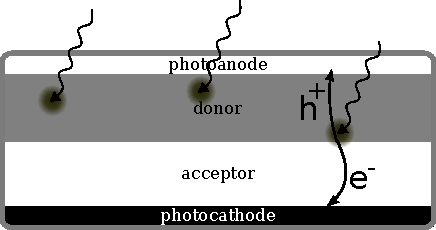
\includegraphics[width=0.5\textwidth]{bilayer-gray.pdf}
\caption[Structure of a bilayer solar cell.]{Structure of a bilayer solar cell. Only excitons generated near an interface can break in free charges.}
\label{fig:bilayer}
\end{SCfigure}

\paragraph{Active layer morphologies} Early organic solar cells were made only of a single organic material sandwiched between two electrodes,\superfootcite{Chamberlain1983} here the charge generation is dependent on the electric potential coming from electrodes and the efficiencies are poor. 
Then bilayer cells (schematized in Figure~\ref{fig:bilayer}) were developed having a donor (\textit{p}-type semiconductor) and an acceptor (\textit{n}-type material) organic material stratified between electrodes,\superfootcite{Tang1986}\superfootcite{Peumans2000}\superfootcite{Halls1996} in these kind of cells the polythiophene made its entrance in organic photovoltaics.\superfootcite{ADMA:ADMA19950070709} 
The problem with these cells arises from the mechanism of charge photo\-generation in organic materials, which occurs as follows: a photon is absorbed, if the energy is large enough a free electron and a hole are formed, otherwise an exciton\nota{\label{fn:exciton}\textit{exciton}, a bound state of an electron and a hole which are attracted to each other by the electrostatic Coulomb force. It is an electrically neutral quasi-particle that exists in insulators, semiconductors and in some liquids. The exciton is regarded as an elementary excitation of condensed matter that can transport energy without transporting net electric charge. (Wikipedia)} 
is formed. 
A sunlight photon has typically enough energy to create a pair of free charges in inorganic semiconductors. Indeed in organic semiconductors the band gap\nota{\label{fn:bandgap}\textit{band gap energy}, the energy difference between the bottom of the conduction band and the top of the valence band or, from a molecular point of view, the difference between \gls{LUMO} and \gls{HOMO}. } 
is higher and depends also on the molecular properties of the material. The so generated excitons have to reach a donor-acceptor materials interface where the high local electric field breaks them in free charges. However, the diffusion length of an exciton in a semiconducting material (5-\SI{10}{\nm}) prior to its dissipative recombination is typically less than the optical absorption length (\SI{\approx50}{\nm}), then a bilayer approach can't have both high absorption and high exciton dissociation efficiencies. 
A possible solution is to greatly increase the interface inter\-dispersing the acceptor and donor materials and obtaining a bulk heterojunction,\superfootcite{Yu1995}\superfootcite{Saunders2008} schematized in Figure~\ref{fig:bhj}. An excessive dispersion could avoid the semi-crystallization in nano\-domains needed for a good charge mobility. Moreover when two opposite charges are formed in the middle of the active layer, they need two continuous pathways to reach the appropriate electrode, thus the presence of segregated domains negatively affects the efficiency, trapping the charges.

\begin{SCfigure}[][tbp]%bhj
\centering
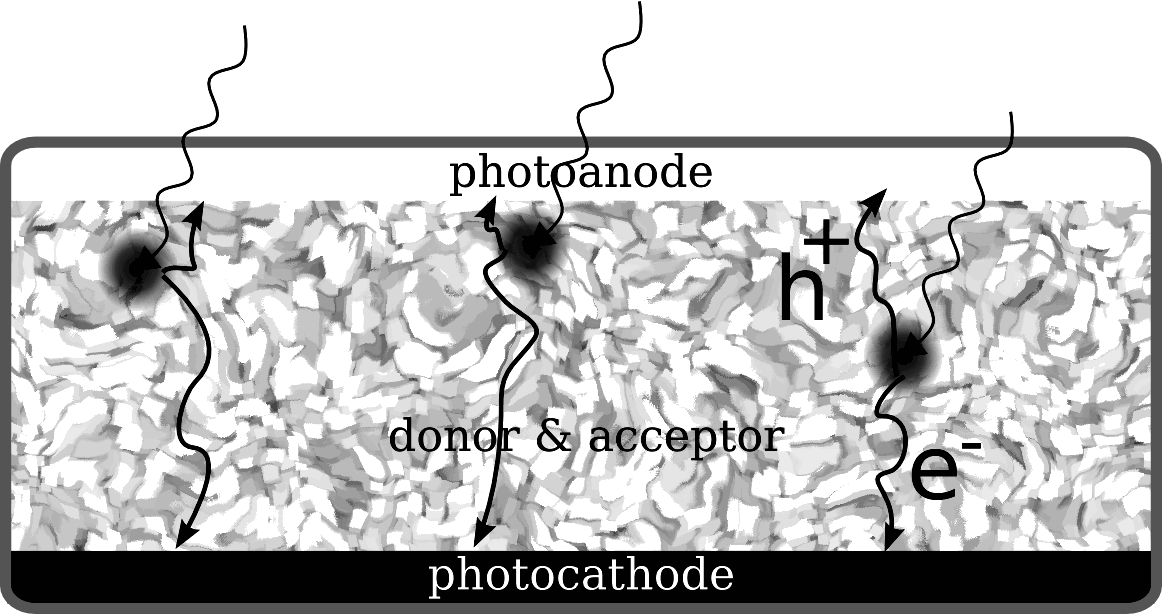
\includegraphics[width=0.5\textwidth]{bhj.png}
\caption{Structure of a bulk heterojunction solar cell.}
\label{fig:bhj}
\end{SCfigure}

\paragraph{Polythiophene in photovoltaics} \Gls{P3HT} in blend with modified fullerene \gls{PCBM} is the reference standard in organic photovoltaics. The role of polythiophene is to absorb the sunlight, transport the generated exciton to the materials interface, donate an electron to \gls{PCBM} and transport the resulting hole towards the anode, while electrons move through \gls{PCBM}. 
A reduced band gap would be highly favorable for absorbing also the low energy portion of the sunlight spectrum. The conjugation length (and then the regioregularity which depends upon the polymerization method) influences the band gap. In recent years many alternating polymers based on thiophene were synthesized with a low band gap. For these polymers a controlled living polymerization method isn't reported yet.

\paragraph{Block copolymers} Unfortunately the materials dispersed in a bulk heterojunction solar cell are usually immiscible, this means that they tend to segregate in two phases over time, reducing the inter\-facial area. In order to compatibilize the acceptor and donor materials, an amphiphilic surfactant can be added.\superfootcite{Liu2012} 
This would introduce in the system a new molecule which could trap charges or act as an insulating layer. An innovative and promising approach is to use an amphiphilic diblock copolymer as donor material, acting as a surfactant itself. The polar block could be designed to complex the \gls{PCBM} (or other inorganic semiconducting nano\-particles) via electron rich sites\superfootcite{Sary2010a}\superfootcite{Topham2011} or can be covalently bonded to the particles. Tuning the blocks volume (changing the degree of polymerization) and the quantity of \gls{PCBM} is a way to optimize the morphology of the blend. 

\end{section}